\section{Supplementary Results}
\label{app:supplementary}

\subsection{Controlled-Grid Accuracy}
\label{app:grid-accuracy}

Figure~\ref{fig:cg-sets} gives the exact-cell accuracy behind the mean errors of Figure~\ref{fig:grid-mae}, together with the accuracy after AoA is added, on which the comparison of BS placements in Section~\ref{subsec:gain-grid} rests.

\par\medskip\noindent\begin{minipage}{\textwidth}
  \centering
  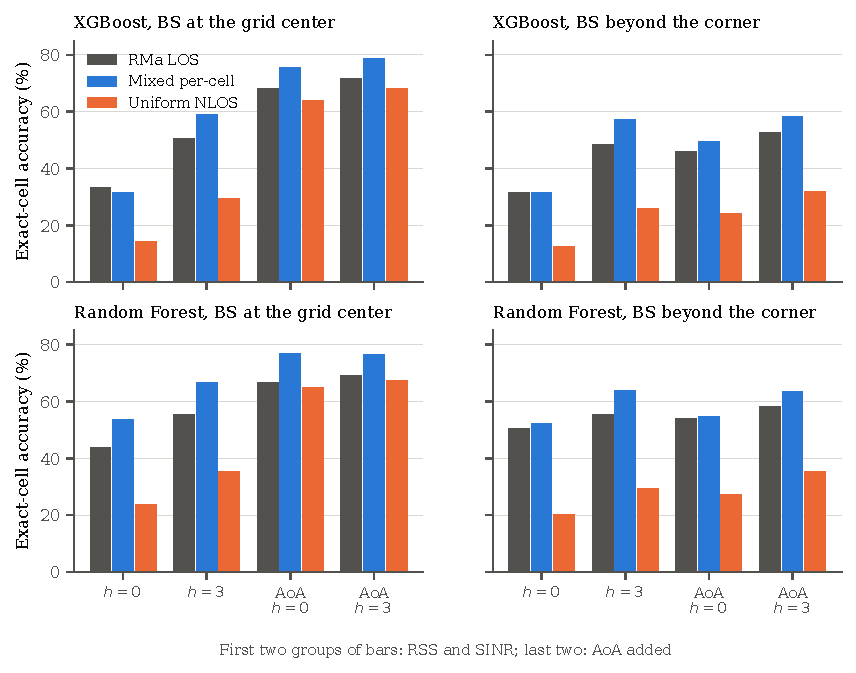
\includegraphics[width=0.82\textwidth]{fig_controlled_grid_sets}
  \captionof{figure}{Controlled grid: exact-cell accuracy at $h=0$ and $h=3$, from RSS and SINR and with AoA added, per classifier, BS placement and propagation setting. Single run per bar.}
  \label{fig:cg-sets}
\end{minipage}\par\medskip
% src: figure_scripts/python/make_figures_followup.py controlled_grid_sets(); comparison_sets.csv

\subsection{Macro-Cell Error Levels}
\label{app:macro-errors}

% src: naive_baseline/uniform_nlos (20 seeds: multi 35.27, single 38.50); pathloss_fit_summary.json (sigma_r 67.94 m at 95 m); seed_repeats_all_models_summary.json knn_h0 (23.38 / 46.17, five splits); followup_2026_10/uniform_nlos XGBoost snap / full (20 seeds: 18.74 / 15.59 multi, 36.33 / 36.51 single)
The constant guess, the ranging resolution of a single RSS reading, and the errors of the trained models are compared per device group in Table~\ref{tab:reference-levels}. A snapshot $k$-NN fingerprint, the classical approach, is worse than the constant guess for single-antenna devices, and the trained models remain about \SI{20}{\meter} apart between the two groups.

\par\medskip\noindent\begin{minipage}{\textwidth}
  \centering
  \captionof{table}{Macro cell, uniform NLOS: reference error levels per device group. The ranging resolution is a standard deviation, not an error.}
  \label{tab:reference-levels}
  \small
  \begin{tabular}{@{}lrr@{}}
    \toprule
    Reference & Multi-antenna & Single-antenna \\
    \midrule
    Constant guess~(mean training position, $20$ splits) & \SI{35.3}{\meter} & \SI{38.5}{\meter} \\
    RSS ranging resolution $\sigma_r$ at median range & \SI{68}{\meter} & \SI{68}{\meter} \\
    \midrule
    $k$-NN, $h=0$~(five splits) & \SI{23.4}{\meter} & \SI{46.2}{\meter} \\
    XGBoost, $h=0$~($20$ splits) & \SI{18.7}{\meter} & \SI{36.3}{\meter} \\
    XGBoost, $h=5$~($20$ splits) & \SI{15.6}{\meter} & \SI{36.5}{\meter} \\
    \bottomrule
  \end{tabular}
\end{minipage}\par\medskip

% src: diagnostics_2026_10/baseline_uniform_nlos/errors_first_seed.npz (seed 42); per_seed.xgboost.full (multi within 10 m 34 %, within 20 m 71 %, p50 13.7, p90 29.5; single 7 %, 21 %, 34.7, 59.1)
\par\medskip\noindent\begin{minipage}{\textwidth}
  \centering
  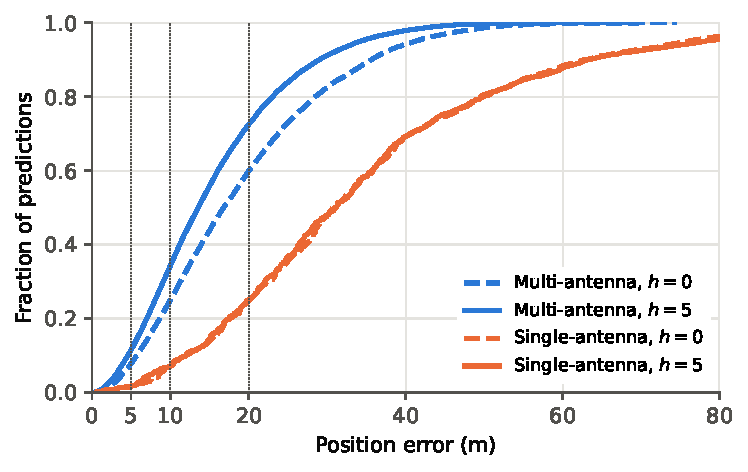
\includegraphics[width=0.65\textwidth]{fig_error_cdf}
  \captionof{figure}{Macro cell: distribution of position error per device group, XGBoost at $h=0$ and $h=5$, one split.}
  \label{fig:error-cdf}
\end{minipage}\par\medskip
% src: figure_scripts/python/make_figures_diagnostic.py error_cdf()
\par\medskip\noindent\begin{minipage}{\textwidth}
  \centering
  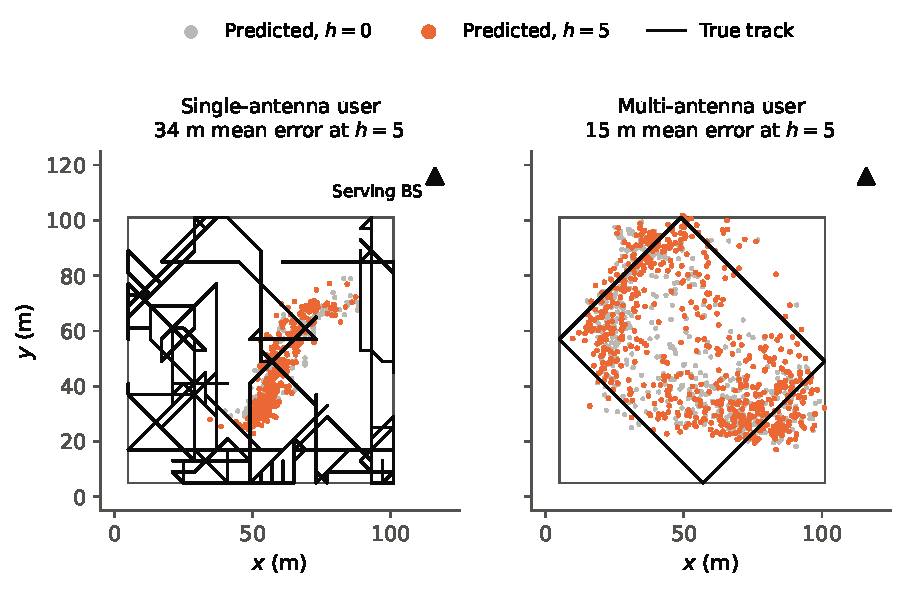
\includegraphics[width=0.75\textwidth]{fig_trajectories}
  \captionof{figure}{Macro cell: true track and predicted positions of the median single-antenna~(left) and multi-antenna~(right) test user, XGBoost at $h=0$ and $h=5$, one split.}
  \label{fig:trajectories}
\end{minipage}\par\medskip
% src: figure_scripts/python/make_figures_diagnostic.py trajectories(); diagnostics_2026_10/baseline_uniform_nlos/errors_first_seed.npz (seed 42; users 250 and 27)

\subsection{Per-Model History Gain in the Macro Cell}

Figure~\ref{fig:history-by-group} shows how the macro-cell gain builds with history depth, Table~\ref{tab:history-gain} gives the per-model values behind Figure~\ref{fig:history-gain-ci}, and Table~\ref{tab:supp-retune} gives the re-tuning check of Section~\ref{subsec:gain-macro}.

% src: history_sweep_all_models_summary.json curves (seed 42, multi_mae by depth); deep_history_sweep_trees_summary.json
\par\medskip\noindent\begin{minipage}{\textwidth}
  \centering
  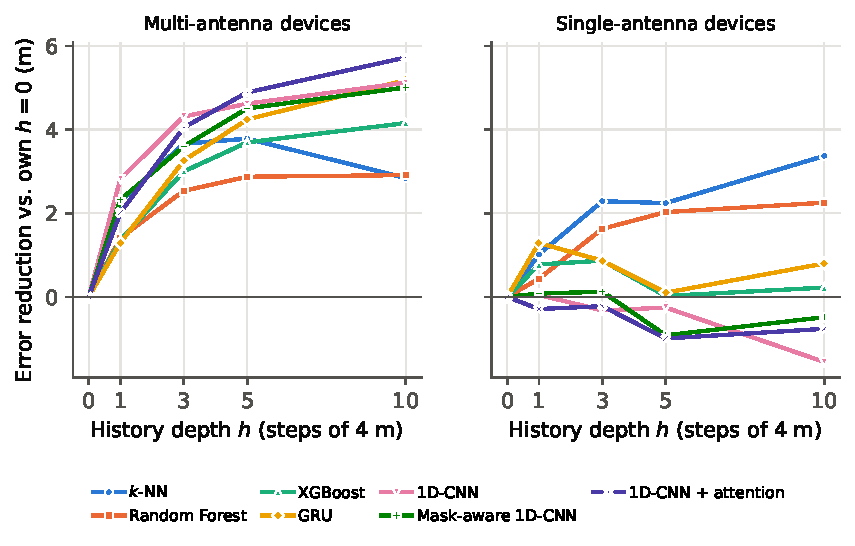
\includegraphics[width=0.85\textwidth]{fig_history_by_group}
  \captionof{figure}{Macro cell: error reduction against each model's own $h=0$ input as history depth grows, per device group, single split.}
  \label{fig:history-by-group}
\end{minipage}\par\medskip
% src: figure_scripts/python/make_figures.py history_by_group(); history_sweep_all_models_summary.json

\par\medskip\noindent\begin{minipage}{\textwidth}
  \centering
  \captionof{table}{Macro cell, uniform NLOS: error at $h=0$ and seed-paired gain from $h=0$ to $h=5$ per model and device group, with \SI{95}{\percent} Student-$t$ intervals, and cost of one run.}
  \label{tab:history-gain}
  \small
  \begin{tabular}{@{}lrrrrrr@{}}
    \toprule
     & \multicolumn{2}{c}{Multi-antenna devices} & \multicolumn{2}{c}{Single-antenna devices} & \multicolumn{2}{c}{Cost} \\
    \cmidrule(lr){2-3}\cmidrule(lr){4-5}\cmidrule(l){6-7}
    Model & Error, $h=0$ & Gain & Error, $h=0$ & Gain & Training & ms per 1000 \\
    \midrule
    $k$-NN & \SI{23.4}{\meter} & \SI{3.77 +- 0.47}{\meter} & \SI{46.2}{\meter} & \SI{-0.11 +- 3.28}{\meter} & \SI{1}{\second} & $577$ \\
    Random Forest$^\ast$ & \SI{18.8}{\meter} & \SI{2.75 +- 0.08}{\meter} & \SI{36.8}{\meter} & \SI{0.42 +- 0.39}{\meter} & \SI{34}{\second} & $102$ \\
    XGBoost$^\ast$ & \SI{18.7}{\meter} & \SI{3.15 +- 0.12}{\meter} & \SI{36.3}{\meter} & \SI{-0.18 +- 0.34}{\meter} & \SI{4}{\second} & $1.7$ \\
    GRU & \SI{19.3}{\meter} & \SI{3.54 +- 0.94}{\meter} & \SI{36.7}{\meter} & \SI{-0.26 +- 1.08}{\meter} & \SI{166}{\second} & $31$ \\
    1D-CNN & \SI{19.5}{\meter} & \SI{3.73 +- 1.20}{\meter} & \SI{36.0}{\meter} & \SI{-1.16 +- 2.59}{\meter} & \SI{197}{\second} & $14$ \\
    Mask-aware 1D-CNN & \SI{19.3}{\meter} & \SI{3.47 +- 1.06}{\meter} & \SI{34.8}{\meter} & \SI{0.25 +- 1.16}{\meter} & \SI{182}{\second} & $18$ \\
    1D-CNN + attention & \SI{19.5}{\meter} & \SI{4.06 +- 1.05}{\meter} & \SI{35.9}{\meter} & \SI{-1.39 +- 4.65}{\meter} & \SI{212}{\second} & $23$ \\
    \bottomrule
    \multicolumn{7}{@{}l}{\footnotesize $^\ast$~$20$ user splits; all other models five.}
  \end{tabular}
\end{minipage}\par\medskip
% src: errors and gains recomputed by figure_scripts/fig_history_gain_ci.m from data/seed_repeats_uniform_nlos.json (five splits) and data/followup20_uniform_nlos.json (20 splits; RF h=0 18.76 / 36.80, XGB 18.74 / 36.33); cost: master_benchmark_rerun_summary.json scorecard (train_time_sec, latency_ms_per_1k; k-NN cost row is the h=5 model)

\par\medskip\noindent\begin{minipage}{\textwidth}
  \centering
  \captionof{table}{Macro cell: overall mean error~(m) with fixed hyperparameters and with hyperparameters re-tuned at each depth on training users only, single split.}
  \label{tab:supp-retune}
  \small
  \begin{tabular}{@{}lrrrr@{}}
    \toprule
     & \multicolumn{2}{c}{XGBoost} & \multicolumn{2}{c}{Random Forest} \\
    \cmidrule(lr){2-3}\cmidrule(l){4-5}
    Depth & Fixed & Re-tuned & Fixed & Re-tuned \\
    \midrule
    $h=0$ & 22.35 & 21.91 & 22.11 & 22.05 \\
    $h=1$ & 21.12 & 21.20 & 20.91 & 20.84 \\
    $h=3$ & 19.80 & 19.66 & 19.77 & 19.81 \\
    $h=5$ & 19.43 & 19.07 & 19.42 & 19.40 \\
    $h=10$ & 19.03 & 18.97 & 19.34 & 19.30 \\
    \bottomrule
  \end{tabular}
\end{minipage}\par\medskip
% src: xgb_per_h_retune_summary.json, rf_per_h_retune_summary.json (as transcribed in FINAL_REPORT.md §5.5)

\subsection{Propagation and Interference}
\label{app:propagation}

% src: mixed_propagation_2026_09/pathloss_fit_summary.json zones.LOS (gamma 2.578, sigma 7.67 dB, R^2 0.261), zones.NLOS (gamma 3.595, sigma 11.89 dB, R^2 0.069); followup_2026_10/mixed_propagation/region_gain_did_vs_uniform.json (20 seeds: gap 1.81 +- 0.27 uniform, 1.54 +- 0.24 mixed; difference -0.27 +- 0.25; RF -0.01 +- 0.18)
In the mixed-propagation realization, a path-loss fit gives $\gamma = 2.58$ and a shadowing spread of \SI{7.7}{\decibel} in the LOS regions, against $\gamma = 3.60$ and \SI{11.9}{\decibel} in the NLOS regions. History lowers the multi-antenna error more in the LOS regions; however, the gap between the regions is the same in the uniform-NLOS realization of the same walks, which contains no LOS~(Figure~\ref{fig:los-nlos}), and its difference between the two realizations, \SI{-0.27 +- 0.25}{\meter} for XGBoost, is not distinguishable from zero. Table~\ref{tab:no-interference} gives the effect of removing the two interfering BSs.

\par\medskip\noindent\begin{minipage}{\textwidth}
  \centering
  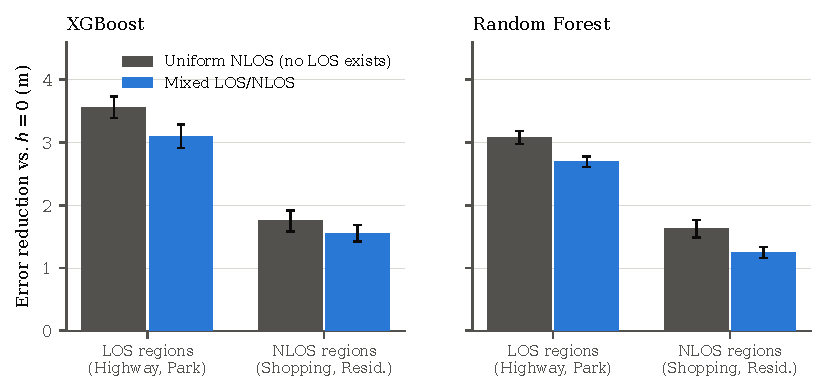
\includegraphics[width=0.8\textwidth]{fig_region_control}
  \captionof{figure}{Macro cell: reduction in multi-antenna error from history in the LOS and NLOS regions of the mixed realization and in the same regions of the uniform-NLOS realization. Seed-paired means over $20$ user splits with \SI{95}{\percent} Student-$t$ intervals.}
  \label{fig:los-nlos}
\end{minipage}\par\medskip
% src: figure_scripts/python/make_figures_followup.py region_control()

\par\medskip\noindent\begin{minipage}{\textwidth}
  \centering
  \captionof{table}{Macro cell: multi-antenna error at $h=0$ and gain from history, with and without the two interfering BSs, over $20$ user splits with \SI{95}{\percent} Student-$t$ intervals.}
  \label{tab:no-interference}
  \small
  \begin{tabular}{@{}llrrrr@{}}
    \toprule
    & & \multicolumn{2}{c}{Error at $h=0$} & \multicolumn{2}{c}{Gain from history} \\
    \cmidrule(lr){3-4}\cmidrule(l){5-6}
    Dataset & Model & with & without & with & without \\
    \midrule
    Uniform NLOS & XGBoost & $18.74$ & $19.30$ & $3.15 \pm 0.12$ & $3.44 \pm 0.17$ \\
    Uniform NLOS & Random Forest & $18.76$ & $19.34$ & $2.75 \pm 0.08$ & $3.15 \pm 0.11$ \\
    Mixed & XGBoost & $17.48$ & $18.46$ & $2.75 \pm 0.15$ & $3.15 \pm 0.17$ \\
    Mixed & Random Forest & $17.15$ & $18.14$ & $2.36 \pm 0.08$ & $2.80 \pm 0.09$ \\
    \bottomrule
  \end{tabular}
\end{minipage}\par\medskip
% src: followup_2026_10/no_interference/{uniform_nlos,mixed_propagation}/history_mechanism_followup_summary.json (20 seeds)
